%%%%%%%%%%%%%%%%%%%%%%%%%%%%%%%%%%%%%%%%%
% Jacobs Landscape Poster
% LaTeX Template
% Version 1.1 (14/06/14)
%
% Created by:
% Computational Physics and Biophysics Group, Jacobs University
% https://teamwork.jacobs-university.de:8443/confluence/display/CoPandBiG/LaTeX+Poster
% 
% Further modified by:
% Nathaniel Johnston (nathaniel@njohnston.ca)
%
% This template has been downloaded from:
% http://www.LaTeXTemplates.com
%
% License:
% CC BY-NC-SA 3.0 (http://creativecommons.org/licenses/by-nc-sa/3.0/)
%
%%%%%%%%%%%%%%%%%%%%%%%%%%%%%%%%%%%%%%%%%

%----------------------------------------------------------------------------------------
%	PACKAGES AND OTHER DOCUMENT CONFIGURATIONS
%----------------------------------------------------------------------------------------

\documentclass[final]{beamer}
\documentclass[conference]{IEEEtran}

% Make latex understand and use the typographic
% rules of the language used in the document.
\usepackage[english]{babel}
\usepackage[utf8]{inputenc}
% Choose the font encoding
\usepackage[T1]{fontenc}

% Use colour in tables
\usepackage[table]{xcolor}
\usepackage{array}
\usepackage{multirow}

% load a colour package
\usepackage{xcolor}
\definecolor{aaublue}{RGB}{33,26,82}% dark blue

% The standard graphics inclusion package
\definecolor{white}{RGB}{255,255,255} % define color white
\usepackage{graphicx}

% Set up how figure and table captions are displayed
\usepackage{caption}
\captionsetup{
  font=footnotesize,% set font size to footnotesize
  labelfont=bf % bold label (e.g., Figure 3.2) font
}

% Enable row combination in tables
\usepackage{multirow}

% Make space between table lines and text
\renewcommand{\arraystretch}{1.5}

% Make the standard latex tables look so much better
\usepackage{array,booktabs}



%%%%%%%%%%%%%%%%%%%%%%%%%%%%%%%%%%%%%%%%%%%%%%%%
% Mathematics
%%%%%%%%%%%%%%%%%%%%%%%%%%%%%%%%%%%%%%%%%%%%%%%%
% Defines new environments such as equation,
% align and split 
\usepackage{amsmath}
\usepackage{relsize}
% Adds new math symbols
\usepackage{amssymb}
% Use theorems in your document
% The ntheorem package is also used for the example environment
% When using thmmarks, amsmath must be an option as well. Otherwise \eqref doesn't work anymore.
\usepackage[framed,amsmath,thmmarks]{ntheorem}
\usepackage{cancel}

%%%%%%%%%%%%%%%%%%%%%%%%%%%%%%%%%%%%%%%%%%%%%%%%
% Page Layout
%%%%%%%%%%%%%%%%%%%%%%%%%%%%%%%%%%%%%%%%%%%%%%%%


%%%%%%%%%%%%%%%%%%%%%%%%%%%%%%%%%%%%%%%%%%%%%%%%
% Bibliography
%%%%%%%%%%%%%%%%%%%%%%%%%%%%%%%%%%%%%%%%%%%%%%%%
%%setting references (using numbers) and supporting i.a. Chicargo-style:
\usepackage{etex}
\usepackage{etoolbox}
\usepackage{keyval}
\usepackage{ifthen}
\usepackage{url}
\usepackage{csquotes}
\usepackage[backend=biber, url=true, doi=true, citestyle=ieee, bibstyle=ieee, sorting=none]{biblatex}
\addbibresource{setup/bibliography.bib}

%%%%%%%%%%%%%%%%%%%%%%%%%%%%%%%%%%%%%%%%%%%%%%%%
% Misc
%%%%%%%%%%%%%%%%%%%%%%%%%%%%%%%%%%%%%%%%%%%%%%%%

%%% Enables the use FiXme refferences. Syntax: \fxnote{...} %%%
\usepackage[footnote, draft, english, silent, nomargin]{fixme}
%With "final" instead of "draft" an error will ocure for every FiXme under compilation.

%%% allows use of lorem ipsum (generate i.e. pagagraph 1 to 5 with \lipsum[1-5]) %%%
\usepackage{lipsum}

%%% Enables figures with text wrapped tightly around it %%%
\usepackage{wrapfig}

\usepackage{float}
\usepackage{caption}
\usepackage{subcaption}
\usepackage{siunitx}
\sisetup{decimalsymbol=comma}
\sisetup{detect-weight}

\usepackage{enumitem}
%\usepackage[citestyle=authoryear,natbib=true]{biblatex}

% Figures - TIKZ
\usepackage{tikz}
\usetikzlibrary{shapes,arrows}
\usepackage[americanresistors,americaninductors,americancurrents, americanvoltages]{circuitikz}

% Wall of text logo
\newcommand{\walloftextalert}[0]{\includegraphics[width=\textwidth]{walloftext.png}}

\usepackage{pdfpages}
\usepackage{lastpage}
\usepackage{epstopdf}

\setlength{\headheight}{21pt}

\hfuzz=\maxdimen
\tolerance = 10000
\hbadness  = 10000

\usepackage{siunitx}
\graphicspath{{./figures/}}% package inclusion and set up of the document

%%%%%%%%%%%%%%%%%%%%%%%%%%%%%%%%%%%%%%%%%%%%%%%%%%%%%
%             UNITS, EQUATIONS AND TEXT             %
%%%%%%%%%%%%%%%%%%%%%%%%%%%%%%%%%%%%%%%%%%%%%%%%%%%%%
%Units:
\newcommand{\unit}[1]{&& \left[\si{#1}\right]} %\newcommand{\unit}[1]{[\si{#1}]}             <<| Use these if you want uations to be
\newcommand{\unitWh}[1]{[\si{#1}]}             %\newcommand{\eq}[2]{&&\si{#1} &= \si{#2}&&}  <<| centered.. .. will appear scrambled
\newcommand{\numUnit}[1]{\ \si{#1}&}           %                                               | from one equation to the next though..
%Equation:                                     %                                               | and does not work with long equations.. :/
\newcommand{\eq}[2]{\si{#1} &= \si{#2}}
\newcommand{\arw}{&& &\Updownarrow&&}
\newcommand{\eqOne}[2]{\si{#1} &= \si{#2} &\nonumber\\}
\newcommand{\eqTwo}[1]{&\ \ \ \ \si{#1}& \nonumber\\}
\newcommand{\eqThree}[1]{&\ \ \ \ \si{#1}&}
%Text:
\newcommand{\tx}[1]{\text{#1}}
%Vectors
\renewcommand{\vec}[1]{\boldsymbol{\mathbf{#1}}}
%Vertical line in equations ie. |_x=y (whereTwo stacks two equalities at the line)
\newcommand{\lineWhere}[1]{ \left.\rule{0cm}{.5cm}\right\vert\rule{0cm}{.4cm}_{\substack{\rule{0cm}{.15cm}\\ \si{#1} }} }
\newcommand{\lineWhereTwo}[2]{ \left.\rule{0cm}{.67cm}\right\vert\rule{0cm}{.5cm}_{\substack{\si{#1} \rule{0cm}{.19cm}\\\vspace{-.1cm}\\ \si{#2}}} }

%%%%%%%%%%%%%%%%%%%%%%%%%%%%%%%%%%%%%%%%%%%%%%%%%%%%%
%                 TIKZ SETTINGS                     %
%%%%%%%%%%%%%%%%%%%%%%%%%%%%%%%%%%%%%%%%%%%%%%%%%%%%%
%\usetikzlibrary{arrows.meta}
\tikzset{
  block/.style    = {draw, thick, rectangle,
                     minimum height = 2.1em,
                     minimum width = 1.7em},
  sum/.style      = {draw, circle, inner sep=1.5pt},
}

%%%%%%%%%%%%%%%%%%%%%%%%%%%%%%%%%%%%%%%%%%%%%%%%%%%%%
%               WHERE, AFTER MATH                   %
%%%%%%%%%%%%%%%%%%%%%%%%%%%%%%%%%%%%%%%%%%%%%%%%%%%%%
\usepackage{xifthen}

\newenvironment{where}{\par\vspace{-4mm}\noindent\ignorespaces Where:\\}{\\}
\newcommand{\va}[3]
{
  \begin{tabular}{p{10pt} p{145pt} l}
    { $#1$ } & { #2 } & \ifthenelse{\isempty{ #3 }}  {}  {[{\si{#3}}]} \\
  \end{tabular}\\
}% my new macros

\usepackage[scale=1.24]{beamerposter} % Use the beamerposter package for laying out the poster

\usetheme{confposter} % Use the confposter theme supplied with this template

%\setbeamercolor{block title}{fg=black,bg=white} % Colors of the block titles
%\setbeamercolor{block body}{fg=black,bg=white} % Colors of the body of blocks
%\setbeamercolor{block alerted title}{fg=white,bg=dblue!70} % Colors of the highlighted block titles
\setbeamercolor{block alerted body}{fg=black,bg=white} % Colors of the body of highlighted blocks
% Many more colors are available for use in beamerthemeconfposter.sty

%-----------------------------------------------------------
% Define the column widths and overall poster size
% To set effective sepwid, onecolwid and twocolwid values, first choose how many columns you want and how much separation you want between columns
% In this template, the separation width chosen is 0.024 of the paper width and a 4-column layout
% onecolwid should therefore be (1-(# of columns+1)*sepwid)/# of columns e.g. (1-(4+1)*0.024)/4 = 0.22
% Set twocolwid to be (2*onecolwid)+sepwid = 0.464
% Set threecolwid to be (3*onecolwid)+2*sepwid = 0.708

\newlength{\sepwid}
\newlength{\onecolwid}
\newlength{\twocolwid}
\newlength{\threecolwid}
\setlength{\paperwidth}{48in} % A0 width: 46.8in
\setlength{\paperheight}{36in} % A0 height: 33.1in
\setlength{\sepwid}{0.024\paperwidth} % Separation width (white space) between columns
\setlength{\onecolwid}{0.23\paperwidth} % Width of one column
\setlength{\twocolwid}{0.42\paperwidth} % Width of two columns
\setlength{\threecolwid}{0.708\paperwidth} % Width of three columns
\setlength{\topmargin}{-0.5in} % Reduce the top margin size

%-----------------------------------------------------------

\usepackage{graphicx}  % Required for including images

\usepackage{booktabs} % Top and bottom rules for tables


%----------------------------------------------------------------------------------------
%	TITLE SECTION 
%----------------------------------------------------------------------------------------

\title{Attitude and position control of a quadcopter in a networked \\	distributed system} % Poster title

\author{\textit{Alejandro Alonso García, Amalie V. Petersen, Andrea Victoria Tram Løvemærke,\\ Niels Skov Vestergaard, Noelia Villarmarzo Arruñada} - Group 733} % Author(s)

\institute{	Email: [aalons16] [apet13] [alavem13] [nveste12] [nvilla16] @student.aau.dk} % Institution(s)

\addtobeamertemplate{headline}{} 
{
	\begin{tikzpicture}[remember picture,overlay] 
	\node [shift={(-15 cm,-11cm)}] at (current page.north east) {\includegraphics[height=9cm]{figures/aau_logo_cropped}}; 
	\end{tikzpicture} 
}
%----------------------------------------------------------------------------------------

\begin{document}

\addtobeamertemplate{block end}{}{\vspace*{1ex}} % White space under blocks
\addtobeamertemplate{block alerted end}{}{\vspace*{1ex}} % White space under highlighted (alert) blocks

\setlength{\belowcaptionskip}{1ex} % White space under figures
\setlength\belowdisplayshortskip{1ex} % White space under equations

\begin{frame}[t] % The whole poster is enclosed in one beamer frame

\begin{columns}[t] % The whole poster consists of three major columns, the second of which is split into two columns twice - the [t] option aligns each column's content to the top

\begin{column}{\sepwid}\end{column} % Empty spacer column

\begin{column}{\onecolwid} % The first column

%----------------------------------------------------------------------------------------
%	INTRODUCTION
%----------------------------------------------------------------------------------------
\begin{block}{Introduction}
\section{Introduction}
% no \IEEEPARstart
%Present topic - uses of drones in reality context, chosen because it is a control challenge, rather than revolutionary.
In the last years, the interest for quadcopters has increased due to the great possibilities they offer. Among these, the most well-known ones are surveillance, inspection of big structures and search and rescue missions in difficult environments \cite{droneuses}.

The quadcopter constitutes a control challenge due to its unstable nature and coupled behavior. The system has 6 degrees of freedom, the 3 position coordinates and the 3 orientations, and there are only four actuation variables which are the motor rotational speeds. The dimension of the problem is explained by McKerrow in \cite{draganflyer}.

%Previous Approaches - examples of what others have done to obtain similar goals of stabilization like we pursue. What have others done differently than we plan to do to obtain the same end result.
The control of a quadcopter has been addressed many times in the recent years. In Mian et al. \cite{backstepping} the quadcopter is controlled using a back-stepping technique and non-linear controllers. Other way of solving the issue is presented in Tayebi et al. \cite{quaternionsPD} in which the quadcopter attitude is modeled using quaternions and controlled with a PD based controller. In \cite{MianWang}, Mian and Yang model the system using its dynamic equations and use non linear controllers to achieve a steady flight while in Mokhtari et al. \cite{GHinf} the system is controlled by a mixture of a robust feedback linearizion and a linear GH$_{\infty}$.

%Describe our approach shortly.
The approach presented here models the quadcopter by a first principles method. This approach yields a non linear model that describes the attitude and translational behavior of the quadcopter. The model is then linearized around an equilibrium point, which is chosen to be in hovering position. With the linearized equations, controllers for attitude and translational behaviors are designed. The angular controller is obtained by means of a state space representation while the translational controller is designed using classical control techniques. In the control system, the translational constitutes an outer loop and sets the reference for the attitude controller. Since the sensors are not placed in the quadcopter and the information comes from an external motion tracking system \cite{vicon}, an analysis on how the network could affect the control loop is also presented. In the last part of the paper, the simulations and experimental results of the designed controllers are shown and discussed.
\end{block}

%----------------------------------------------------------------------------------------
%	MODEL
%----------------------------------------------------------------------------------------
\begin{block}{Model}
\section{Model}\label{sec:model}
%Model - Drawing, equations, linear equations.
The quadcopter free body diagram is shown in \autoref{droneDiagram}. 
\begin{figure}[H]
	\centering
	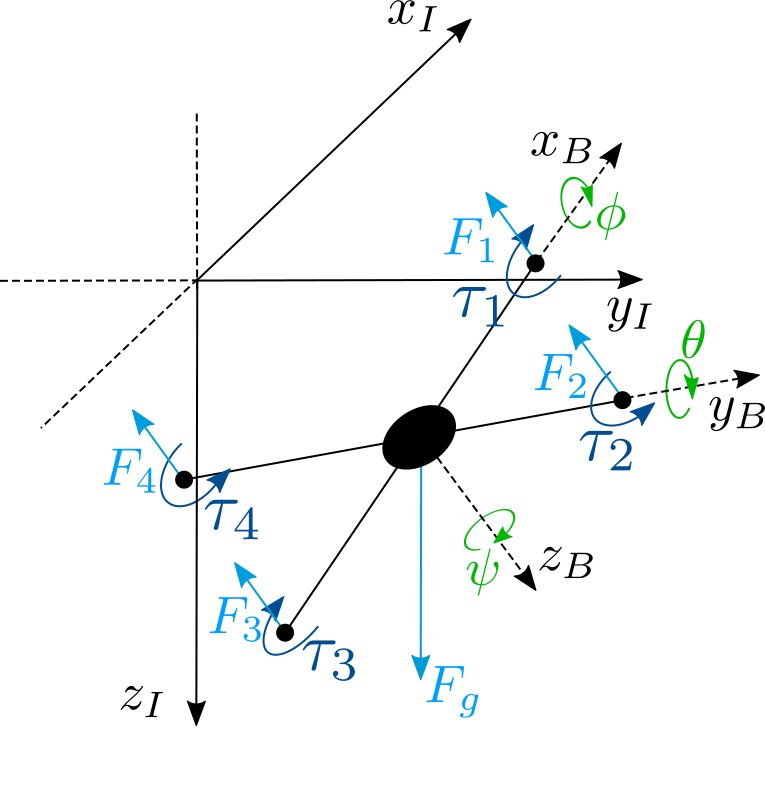
\includegraphics[width=.4\textwidth]{figures/droneDiagram}
	\caption{Forces ($\vec{F}_i$) and torques ($\vec{\tau}_i$) acting on the quadcopter and the positive references chosen for rotations and translations in both inertial and body coordinate frames.}
	\label{droneDiagram}
\end{figure}
%
As it is seen, the system is modeled by using two coordinate frames. The inertial frame is utilized to describe the translational movement while the body frame is attached to the quadcopter and used to characterize its attitude behavior. In the figure, also the positive references for rotational and translational movements are depicted, as well as the main forces and torques acting on the quadcopter. The positive rotations follow a right-hand fashion.

The forces generated in the propeller are readily obtained in the body coordinate frame. In order to represent them in the inertial frame a rotation matrix is used. It is built considering a 123 rotation sequence \cite{rotationmatrix}. This means that any rotation is described as three rotations around the $x_\mathrm{B}$ axis first, then around the $y_\mathrm{B}$ axis and lastly around the $z_\mathrm{B}$ axis. 
 
The dynamic model of the quadcopter is given by three sets of equations. The first describes the motor and the propeller, the second presents the attitude response of the quadcopter and the third explains how the translational variables of the system evolve.

\fxnote{In the modeling section, what are your assumptions? What is the reason for not including model parts such as Gyroscopic torque, Air friction/drag on the quadcopter itself (even though you include it on the propellers), Aerodynamic lift, Mass placement and separation of masses, Coriolis acceleration?}

\subsection{Motor and Propeller}
The four motors in the quadcopter generate a rotation in the propellers that creates the force that lifts the quadcopter. The thrust force can be modeled as proportional to the square of the motor rotational speed. The thrust coefficient for each motor is found experimentally. The units for this coefficient are \si{N s^2 rad^{-2}}
 
The rotation also generates a torque on each motor due to the aerodynamic drag. Drag torque is compensated in the quadcopter by having two of the motors turning in one direction and the two others in the opposite direction. It is as well described as proportional to the square of the rotational speed in terms of a drag coefficient, which is also obtained experimentally. Its units are \si{N m s^2  rad^{-2}}

The expressions for the thrust force and drag torque caused by the rotation of each propeller are
%
\begin{flalign}
	F&=k_{\mathrm{th}}\omega^2\label{eq:thrustForce}\\
	\tau&=k_{\mathrm{d}}\omega^2\label{eq:dragTorque}
\end{flalign}
%
\noindent where $F$ is the thrust force, $k_{th}$ is the thrust coefficient, $\omega$ is the angular speed of the motor, $\tau$ is the drag torque and $k_d$ is the drag coefficient.
%\begin{where}
%  \va{F}{is the thrust force}{N}
%  \va{k_{th}}{is the thrust coefficient}{N\  s^2 \  rad^{-2}}
%  \va{\omega}{is the angular velocity}{rad s^-1}
%  \va{\tau}{is the drag torque}{N m}
%  \va{k_d}{is the drag coefficient}{N \  m\  s^2 \  rad^{-2}}
%\end{where}

These equations are used in the attitude and translational models presented below.
%
\subsection{Attitude Model}
The attitude model equations, which are based on Newton's Second Law for rotational movement, are as follows 
%
\begin{flalign}
	J_x\ddot{\phi}&=k_{\mathrm{th}} (\omega^2_4-\omega^2_2)  L \label{eq:AngleEqVelocities1}\\
	J_y\ddot{\theta}&=k_{\mathrm{th}} (\omega^2_1-\omega^2_3)  L \label{eq:AngleEqVelocities2} \\
	J_z\ddot{\psi}&=k_{\mathrm{d}} (\omega^2_1-\omega^2_2+\omega^2_3-\omega^2_4)\label{eq:AngleEqVelocities3}
\end{flalign}

\noindent where $J_x$, $J_y$ and $J_z$ are the moments of inertia around the three axes of rotation, $\ddot{\phi}$, $\ddot{\theta}$ and $\ddot{\psi}$ are the angular accelerations in roll, pitch and yaw, respectively, $\omega_i$ is the rotational speed of each motor and $L$ is the distance between the center of the quadcopter and the position of the motors.

The expressions above state how the thrust forces and the drag torques generated on the propellers affect the attitude behavior of the quadcopter.  
\subsection{Translational Model}
The equations describing the response of the system along the inertial x, y and z axes are derived from Newton's Second Law of Motion. The forces that act on the system are those from the propellers and the gravitational force. These expressions are
%
\begin{flalign}
     m\ddot{x}_{\mathrm{I}} = &-k_{\mathrm{th}} ({\omega_1}^2+{\omega_2}^2+{\omega_3}^2+{\omega_4}^2) \label{eq:AccelerationEqInertial1}\\
     & \ \times (\cos\phi \sin\theta \cos\psi + \sin\phi\sin\psi)   \nonumber\\
     m \ddot{y}_{\mathrm{I}} = &-k_{\mathrm{th}}({\omega_1}^2+{\omega_2}^2+{\omega_3}^2+{\omega_4}^2) \label{eq:AccelerationEqInertial2}\\
     & \ \times(\cos\phi \sin\theta \sin\psi - \sin\phi \cos\psi)  \nonumber\\
     m\ddot{z}_{\mathrm{I}} = &F_g-k_{\mathrm{th}}\ ({\omega_1}^2+{\omega_2}^2+{\omega_3}^2+{\omega_4}^2) \label{eq:AccelerationEqInertial3}\\
     & \ \times \cos\phi\cos\theta  \nonumber
\end{flalign}
\noindent where $m$ is the mass of the quadcopter, $\ddot{x}_I$, $\ddot{y}_I$ and $\ddot{z}_I$ are the accelerations along the inertial reference frame directions, $\phi$, $\theta$ and $\psi$ are the roll, pitch and yaw angles respectively and $F_g$ is the gravitational force acting on the quadcopter.

It is worth mentioning that, as the thrust forces always point in the negative ${z}_B$ direction, the accelerations along ${x}_{\mathrm{I}}$ and ${y}_{\mathrm{I}}$ directions are zero when pitch and roll angles are zero.

\subsection{Linearization}
The model equations are linearized using the first order Taylor approximation around an equilibrium point of the system. The chosen point is the hovering position, which implies that the attitude and translational accelerations and velocities are zero. The angular position of the quadcopter is also part of the point around which the linearization is made, and it is also set to zero in the three angles.

Choosing a zero acceleration linearization point along the ${z}_{\mathrm{I}}$ axis yields an equilibrium rotational speed so that the necessary thrust is generated to compensate for the gravitational force. The relation is expressed as\fxnote{Should we use the same $\overline{\omega}$?}
\begin{flalign}
    \overline{\omega}_i=\sqrt{\frac{mg}{4k_{th}}}
    \label{eq:equilibriumomegas}
\end{flalign}
The resulting equations for the attitude model after the linearization are 
\begin{flalign}
  J_x \Delta\ddot{\phi}  = &2 k_{\mathrm{th}} L {\overline{\omega}_4} \Delta \omega_4 - 2\ k_{\mathrm{th}} L {\overline{\omega}_2} \Delta \omega_2
  \label{eqAngleLin1} \\
  J_y\Delta\ddot{\theta} =&2 k_{\mathrm{th}} L \overline{\omega}_1 \Delta \omega_1 - 2 k_{\mathrm{th}} L \overline{\omega}_3 \Delta \omega_3
  \label{eqAngleLin2} \\
  J_z\Delta\ddot{\psi}= &2 k_{\mathrm{d}} {\overline{\omega}_1} \Delta \omega_1 - 2 k_{\mathrm{d}}{\overline{\omega}_2} \Delta \omega_2 \label{eqAngleLin3}
  \\ & +\ 2\ k_{\mathrm{d}} {\overline{\omega}_3} \Delta \omega_3 - 2\ k_{\mathrm{d}} {\overline{\omega}_4} \Delta \omega_4\nonumber  
\end{flalign}
\noindent where $\Delta\ddot{\phi}$, $\Delta\ddot{\theta}$ and $\Delta\ddot{\psi}$ are the changes in rotational acceleration from the linearization point, $\overline{\omega}_i$ is the rotational speed of each motor to achieve equilibrium along the $z_\mathrm{I}$ axis and $\Delta \omega_i$ is the change in rotational speed of each motor from the linearization point. 

Similarly, the equations of the translational model are linearized. The result is
\begin{flalign}
  m\Delta\ddot{x}_{\mathrm{I}} =&-k_{\mathrm{th}} ({\overline{\omega}_1}^2+{\overline{\omega}_2}^2+{\overline{\omega}_3}^2+{\overline{\omega}_4}^2) \Delta\theta \label{eq:TransLinearEquations1} \\
  m\Delta\ddot{y}_{\mathrm{I}} = &\ \  \  k_{\mathrm{th}} ({\overline{\omega}_1}^2+{\overline{\omega}_2}^2+{\overline{\omega}_3}^2+{\overline{\omega}_4}^2) \Delta\phi \label{eq:TransLinearEquations2}\\
  m\Delta\ddot{z}_{\mathrm{I}} = &-2 k_{\mathrm{th}}\overline{\omega}_1 \Delta\omega_1 -2 k_{\mathrm{th}} \overline{\omega}_2 \Delta\omega_2 \label{eq:TransLinearEquations3} \\
 &\ \   -2 k_{\mathrm{th}} \overline{\omega}_3 \Delta\omega_3-2 k_{\mathrm{th}} \overline{\omega}_4 \Delta\omega_4 \nonumber 
\end{flalign} 
\noindent where $\Delta\ddot{x_{\mathrm{I}}}$, $\Delta\ddot{y_{\mathrm{I}}}$ and $\Delta\ddot{z_{\mathrm{I}}}$ are the changes in linear acceleration from the linearization point in each direction of the inertial frame and $\Delta \phi$ and $\Delta \theta$ are the changes in roll and pitch from the linearization point, respectively.
\end{block}

%----------------------------------------------------------------------------------------

\end{column} % End of the first column

\begin{column}{\sepwid}\end{column} % Empty spacer column

\begin{column}{\twocolwid} % Begin a column which is two columns wide (column 2)


%----------------------------------------------------------------------------------------
%	CONTROL SOLUTION
%----------------------------------------------------------------------------------------
\begin{block}{Control Solution}
\section{Control}\label{sec:control}\fxnote{Say that we use the network for the design}
The control of the system is divided into two control systems. One handles the attitude and the other controls the translational behavior of the quadcopter. These two are related such that the translational controller sets the references for the angles handled by the inner controller.
\end{block}

%----------------------------------------------------------------------------------------

%----------------------------------------------------------------------------------------
%	RESULTS
%----------------------------------------------------------------------------------------
\begin{alertblock}{Results}
	\section{Results}

The controllers have been simulated in MATLAB Simulink in order to generate results presented in this section. 

The model parameters can be seen in \autoref{ParametersQuadcopter}. All of them have been obtained through test but the moments of inertia, which were calculated with following an analytical procedure.

\begin{table}[H]
    \centering
    \begin{tabular}{c|c|c}
        %------------------------------------------------------------------------------------------
        \textbf{Symbol} &\textbf{Value} &\textbf{Units}\\
        \hline %-----------------------------------------------------------------------------------
        $m$ & 0.996       &$kg$\\
        \hline %-----------------------------------------------------------------------------------
        $L$  &   0.225       & $m$\\
        \hline %-----------------------------------------------------------------------------------
        $J_x$  & 0.01073       & $kg \  m^2$\\
        \hline %-----------------------------------------------------------------------------------
        $J_y$  & 0.01073       & $kg \  m^2$\\
        \hline %-----------------------------------------------------------------------------------
        $J_z$  & 0.02135       & $kg \  m^2$\\
        \hline %-----------------------------------------------------------------------------------
        $k_{th}$  & 1.32922\ $10^{-5}$       & $N \  s^2 \  rad^{-2}$\\
        \hline %-----------------------------------------------------------------------------------
        $k_{d}$  & 9.39741\ $10^{-7}$       & $N \  m \  s^2 \  rad^{-2}$\\
        \hline %-----------------------------------------------------------------------------------
        $\overline{\omega}_i$& 429      & $rad \ s^{-1}$\\
        
    \end{tabular}
    \caption{Parameters used though the analysis and design.}

    \label{ParametersQuadcopter}
\end{table}
The attitude controller is defined chosen feedback and integral poles and the observer poles. These are chosen to be $[-6 -6.2 -6.4 -6.6 -6.8 -7 -7.2 -7.4 -7.6]$ and $[-20 -25 30]$ respectively.

The translation velocity controllers of the x and y translational are $C_{\dot{x}}(s)= -0.1$, $C_{\dot{y}}(s)= 0.1$ and the position ones are $C_x(s)= 0.5$, $C_y(s)= 0.5$. The inner loop proportional controller of the z translational cascade controller is
$C_{\dot{z}}(s)=\frac{-201s+0.8}{s}$ and the outer loop is $C_z=0.9$

This controllers have been discretized using th Tustin method with a sampling period of 30 ms. 

Regarding the network, the mean delay selected is 30 ms and the package loss probability has been set to 0 due to the low sending frequency used in the system.
The simulation results obtained with these parameters and controllers are shown in \autoref{PositionControl}.
\begin{figure}[H]
	\centering
	\includegraphics[scale=0.55]{figures/PositionControl}
	\caption{Position control results in the three inertial axes directions. The references given to the control system are shown with dashed lines.}
	\label{PositionControl}
\end{figure}

The inner attitude controller results are also included and shown in \autoref{AttitudeControl}, so the performance of the attitude control can be evaluated. 
\begin{figure}[H]
	\centering
	\includegraphics[scale=0.55]{figures/AttitudeControl}
	\caption{Attitude control results in the three angles. The references given to the attitude control system are shown with dashed lines.}
	\label{AttitudeControl}
\end{figure}



	The attitude controller is defined by the chosen feedback and integral poles, \\$[-6.0, -6.2, -6.4, -6.6, -6.8, -7.0, -7.2, -7.4, -7.6]$, and  the observer poles, $[-20, -25, -30]$.
	The translation velocity controllers for x and y are $C_{\dot{x}}(s)= -0.1$, $C_{\dot{y}}(s)= 0.1$ and the position ones are $C_x(s)= 0.5$, $C_y(s)= 0.5$. The PI-controller for the z translational velocity is $C_{\dot{z}}(s)=-201\frac{s+0.8}{s}$ and the outer loop P-controller is $C_z=0.9$.
\end{alertblock} 

\end{column} % End of the second column

\begin{column}{\sepwid}\end{column} % Empty spacer column

\begin{column}{\onecolwid} % The third column

%----------------------------------------------------------------------------------------
%	Results
%----------------------------------------------------------------------------------------

%----------------------------------------------------------------------------------------

%----------------------------------------------------------------------------------------
%	DISCUSSION
%----------------------------------------------------------------------------------------
\begin{block}{Discussion}
\section{Discussion}\label{sec:discussion}

The results obtained show both the attitude and simulated position response of the quadcopter. 

It is seen that the controllers track the references even though the network delay and the sampling rate affects their performance. The network limits the designed bandwidths, especially for the attitude controller. This is due to the limited frequency in which the sensor data is obtained from the motion tracking system. A faster response is achievable if on board sensors for acquiring the attitude are utilized.

Experimental results could not be presented for the translational controllers, as it has not been possible to implement them with success in due time. The design is however deemed reasonable, as simulations show that the design should work in reality. The attitude controller is implemented and achieves the given references.

%Experimental results could not be presented for the translational controllers. As the attitude design has been validated with the same simulation and it works in reality, it can be suggested that it is not the design but the implementation of the translational controllers which, at this point in the design process prevents the realization of a flying quadcopter.
%
%Simple model
%Translational 
%The attitude controller tracks the given references in roll and pitch. The network delay 
%It is also worth observing how the attitude controller shows a permanent error with respect to the reference. This is generated as a result of the integral controller design because it assumes a constant reference applied to it. This issue, though, does not affect the final position of the quadcopter.
%\fxnote{why the controllers are slow?, the delay is high}   
\end{block}

%----------------------------------------------------------------------------------------
%	Conclusion
%----------------------------------------------------------------------------------------
\begin{block}{Conclusion}
\section{Conclusion}
The behavior of a quadcopter has been modeled by first principles of physics. A control system has been designed in order to hover and move to a desired position.
The control system has been split into an attitude and a translational controller. The first one has been designed using a state space approach, including state feedback with integral control and a reduced order observer. The translational control system has been designed with a classical control approach and result in three cascade loops, including proportional and PI controllers. 
As the quadcopter uses an external motion tracking system to determine its position and orientation, an analysis of the issues that can arise when having a networked distributed system has been done in order to ensure the control system remains stable. The results obtained from the design show that both the attitude and the translational behavior of the quadcopter has been successfully controlled.

 
\end{block}

%----------------------------------------------------------------------------------------
%	References
%----------------------------------------------------------------------------------------
\begin{block}{References}

\small{\rmfamily{CONTROL BOOK.}} \\
%\nocite{*} % Insert publications even if they are not cited in the poster
%\small{\bibliographystyle{unsrt}
%\bibliography{sample}\vspace{0.75in}}
\printbibliography
\end{block}

%----------------------------------------------------------------------------------------
%	Acknowledgements
%----------------------------
\begin{block}{Acknowledgements}

\small{\rmfamily{Henrik Shøiler, Associated Professor, Aalborg University.\\
Christoffer Sloth, Associated Professor, Aalborg University.}} \\
\end{block}

%----------------------------------------------------------------------------------------

\end{column} % End of the third column

\end{columns} % End of all the columns in the poster
\tikz[remember picture,overlay] \node[opacity=0.7,inner sep=0pt] at (current page.center){\includegraphics[width=\paperwidth,height=\paperheight]{figures/drawing}};
\clearpage
\end{frame} % End of the enclosing frame

\end{document}
